\section{Durchführung}
\label{sec:Durchführung}

Zur Versuchsdurchführung wird eine Hochvakuum-Diode verwendet(s. Abbildung (4)), da die Elektronen sonst mit den Luftmolekülen wechselwirken würden.
In dem Glaskörper, welcher das Vakuum darstellt, befindet sich ein Draht, der erhitzt werden kann. Die damit frei werdenden Elektronen werden mit einem elektrischen Feld, welches zwischen Kathode und Anode herrscht, abgesaugt.
Es fließt nur ein Strom, wenn die Anode gegenüber der Kathode positiv gespannt ist.
\begin{figure}[H]
  \centering
  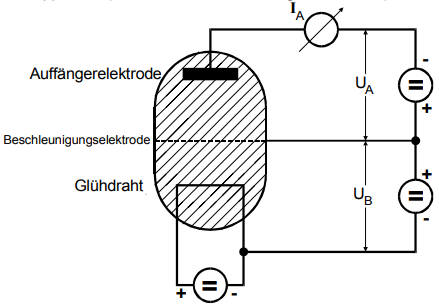
\includegraphics[width=0.8\textwidth]{aufbau.png}
  \caption{Schematischer Aufbau der Messapparatur\cite{kent}.}
  \label{fig:aufbau}
\end{figure}
\noindent Zuerst soll eine Kennlinienschar aus 5 Kennlinen erstellt werden. Dazu wird die Schaltung in Abbildung (5) verwendet. Mit einem Konstantspannungsgerät wird ein Heizstrom von 2,0 - 2,4 $\si{\ampere}$ erzeugt. Die Heizspannung wird mit einem Voltmeter gemessen. An dem Konstantspannungsgerät kann die Anodenspannung geregelt werden.
Für die Kennlinien wird dann die Spannung in mehreren Schritten von 0 bis 250 $\si{\volt}$ und die zugehörige Stromstärke gemessen. Dabei wird der Heizstrom in 0,1 Schritten hochgeschaltet und für jeden Strom die Heizspannung zusätzlich notiert.
Aus der Kennlinienschar wird zuletzt der Sättigunsstrom $I_S$ abgelesen.
\begin{figure}[H]
  \centering
  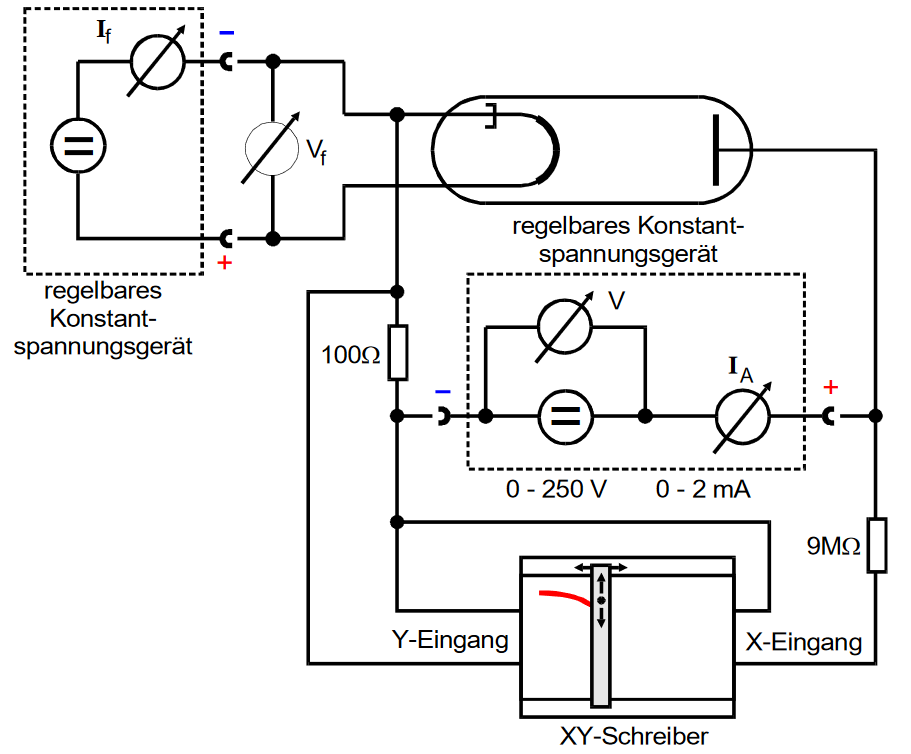
\includegraphics[width=0.8\textwidth]{1.png}
  \caption{Schaltung zur Analyse der Kennlinien\cite{kent}.}
  \label{fig:aufbau}
\end{figure}
Als nächstes wird für die maximal mögliche Heizleistung das Langmuir-Schottkysche Raumladungsgesetz analysiert und der Exponent der Gleichung bestimmt.
Außerdem wird für die maximale Heizleistung die Anlaufkurve bestimmt. Dazu wird die Schaltung aus Abbildung (6) benutzt. Es ist darauf zu achten, dass empfindlichere Messgeräte benötigt werden, und somit genauere Kabel und kurze Verbindungen von Nöten sind.
Der Innenwiderstand des Nanoamperemeters beträgt $R_i = 1 \si{\mega\ohm}$, und der Anlaufstrom erzeugt dort einen Spannungsabfall.
Wieder werden Spannung und zugehörige Stromstärke notiert, und daraus die Kathodentemperatur $T$ bestimmt.
Desweiteren wird aus einer Leistungsbilanz die Kathodentemperatur der Heizleistung aus der ersten Messreihe bestimmt.
Aus der Temperatur und den zugehörigen Stromwerten wird zuletzt die Austrittsarbeit des Kathodenmaterials, welches in diesem Fall Wolfram ist, bestimmt.
\begin{figure}[H]
  \centering
  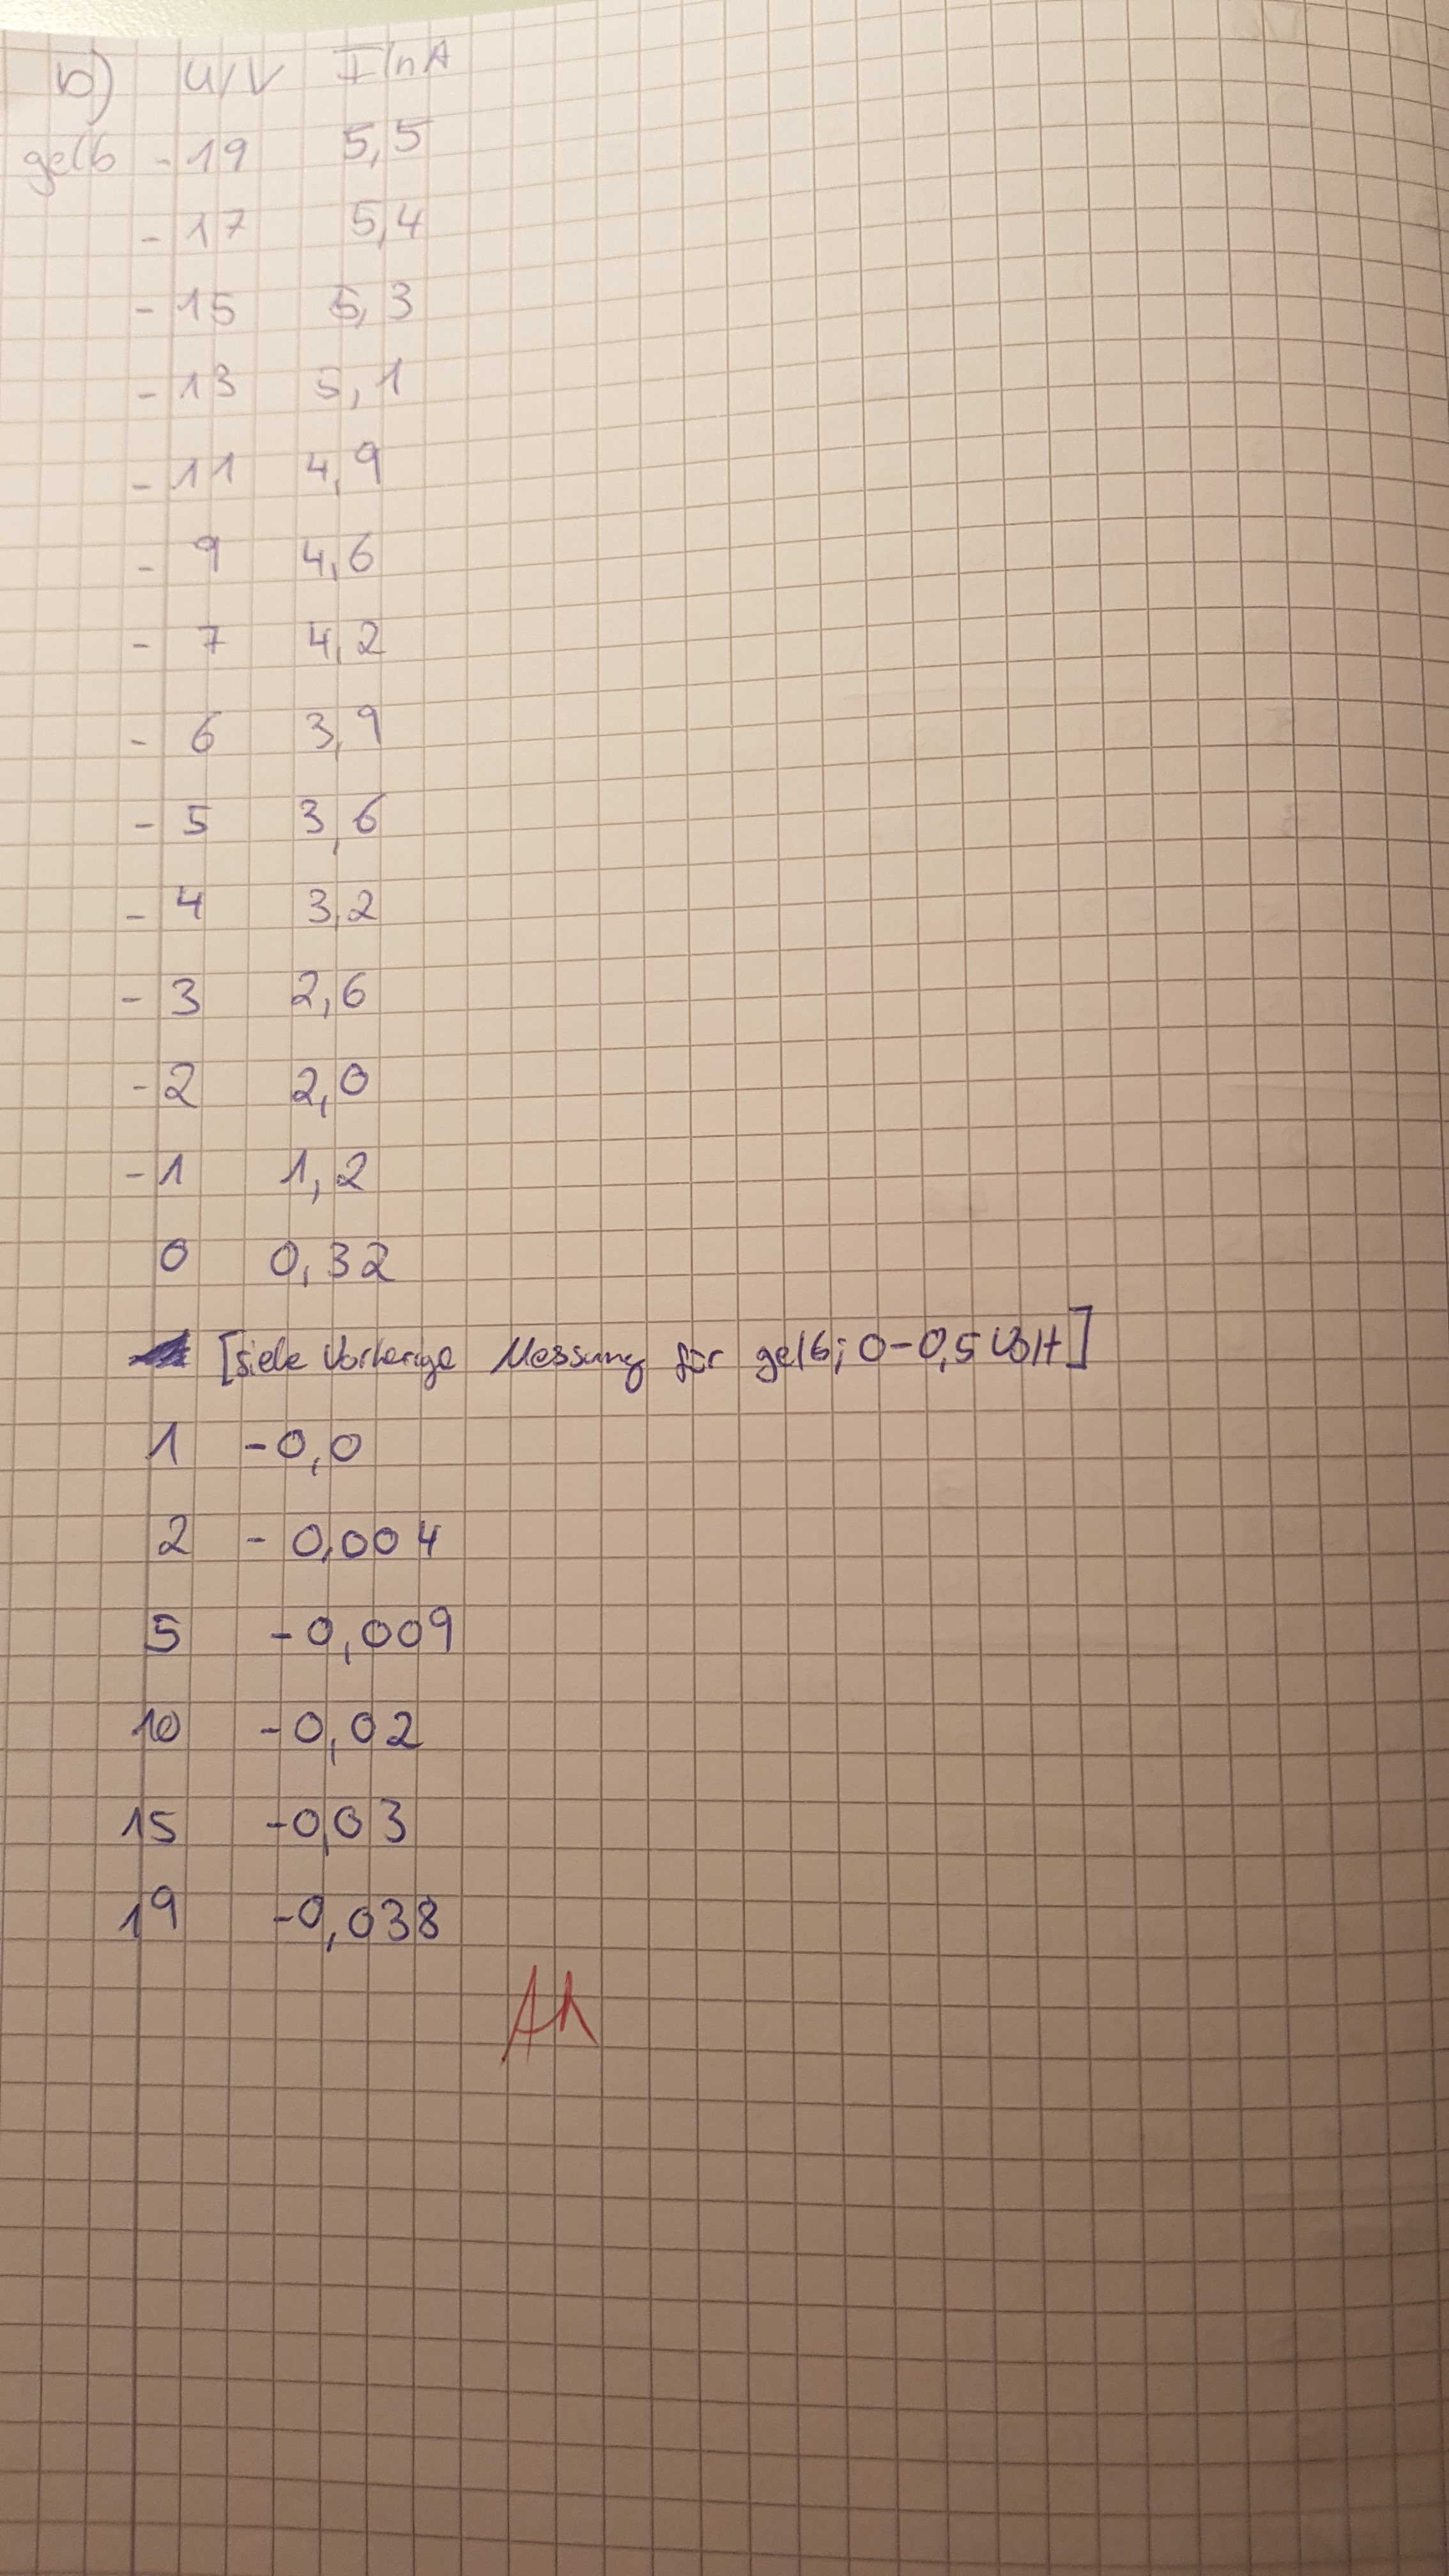
\includegraphics[width=0.8\textwidth]{2.png}
  \caption{Schaltung zur Analyse der Anlaufkurve \cite{kent}.}
  \label{fig:aufbau}
\end{figure}